\scanpage{17}
$x$ en question, ou les $i$ en question) forment un \uline{torseur} sous le groupe $\handwritten{Z^+}=$\deleted{$\handwritten{U\unsure{\cap}}\operatorname{Cent}(u)$}\inserted{$\handwritten{Z\cap U}$}, qui est un groupe
% The lower curved enclosure and its descending leader are distinct from the heavy cancellation.
% The endpoint is placed broadly after unipotent, without assigning it to a precise punctuation stroke.
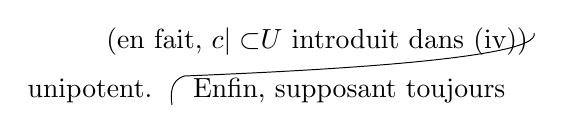
\begin{tikzpicture}[baseline=(unip.base),x=1cm,y=1cm]
\node[anchor=base west,inner sep=0pt] (unip) at (0,0) {unipotent\handwritten{.}};
\node[anchor=base west,inner sep=0pt] at (2.1,0) {Enfin, supposant toujours};
\node[anchor=base west,inner sep=0pt] (cancelnote) at (1.0,.62) {\handwritten{\deleted{(\unsure{en} fait, $\unsure{c|\subset}U$ introduit dans (iv))}}};
\draw[line width=.35pt] ([xshift=2pt,yshift=3pt]cancelnote.east) .. controls ([xshift=5pt,yshift=-7pt]cancelnote.east) and (3.2,.32) .. (2.0,.27) .. controls (1.82,.22) and (1.82,.04) .. (1.84,-.10);
\end{tikzpicture}
% margin note written slanted
\margin{\handwritten{cf plus bas définition de $U$. On a $Z\simeq Z_{\unsure{o|0}}.Z^+$ \deleted{\unsure{Commuté|Commutatif}} (produit $\unsure{\tfrac{1}{2}}$-direct) avec $Z_o=Z\cap L=\operatorname{Cent}(f)$.}}
$e\handwritten{\ne}0$, l'ensemble des $x$ en question est un torseur sous \deleted{$\handwritten{\unsure{\mathfrak{g}|\mathscr{G}}}^{e}=$ (centralisateur de $e$ \deleted{\unsure{dans}} dans $\handwritten{\mathfrak{g}}$)$=\operatorname{Ker}\operatorname{ad}(e)=\operatorname{Lie}\operatorname{Cent}(u)$}\inserted{$\handwritten{\operatorname{Lie}(Z^+)=\mathfrak{g}^{e}\cap\operatorname{Fil}^{1}(\mathfrak{g})}$} (\inserted{\handwritten{torseur}}pour l'addition, i.e. est de la forme $a+\handwritten{\mathfrak{g}}^e$, pour un $a\handwritten{\in\mathfrak{g}}$ convenable)\handwritten{.} \deleted{(et on a $\handwritten{\mathfrak{g}}^{e}\handwritten{\subset\sum}_{k\handwritten{\geq}1}\handwritten{\mathfrak{g}}(k)=\operatorname{Fil}^{1}\handwritten{\mathfrak{g}}$)}

(iii) Soit $x\inserted{\handwritten{\ne0}}$ un élément de Dynkin de $\handwritten{\mathfrak{g}}$, donc associé à un homomorphisme de Dynkin $i:\underline{G}_m\handwritten{\longrightarrow}G$. Alors les éléments\inserted{\handwritten{$e$}} de $\handwritten{\mathfrak{g}}$ tels que $(x,e)$ satisfasse\deleted{nt} aux conditions de (i) forment un ouvert dense\inserted{\handwritten{\deleted{$\unsure{\mathfrak{g}(2)^*}$}}} de $\handwritten{\mathfrak{g}}(2)$ (savoir l'ouvert\inserted{\handwritten{$\mathfrak{g}(2)^*$}} des points $e$ tels que $\operatorname{ad}(e):\handwritten{\mathfrak{g}}(0)\handwritten{\to\mathfrak{g}}(2)$ soit surjectif), \begin{tikzpicture}[baseline=(oldqui.base),x=1cm,y=1cm]
\node[anchor=base west,inner sep=0pt] (oldqui) at (0,0) {\deleted{qui}};
\node[anchor=base west,inner sep=0pt] at (.85,0) {est un};
\node[anchor=base west,inner sep=0pt] (newcelui) at (.05,.60) {\inserted{%
% A typed hyphen is crossed by a separate bowed pen stroke; it is not a typed plus.
\begin{tikzpicture}[baseline=(celui.base)]
\node[anchor=base west,inner sep=0pt] (celui) at (0,0) {Celui};
\node[anchor=base west,inner sep=0pt] (dash) at (celui.base east) {-};
\node[anchor=base west,inner sep=0pt] (ci) at (dash.base east) {ci};
\draw[line width=.5pt] ([xshift=1pt,yshift=6pt]dash.center) .. controls ([xshift=-3pt,yshift=2pt]dash.center) and ([xshift=-3pt,yshift=-2pt]dash.center) .. ([xshift=1pt,yshift=-6pt]dash.center);
\end{tikzpicture}}};
% Thin lower curve joins the raised replacement to the baseline after the cancelled word.
\draw[line width=.35pt] ([xshift=3pt,yshift=1pt]newcelui.east) .. controls ([xshift=3pt,yshift=-9pt]newcelui.east) and (1.1,.29) .. (.82,.26) .. controls (.66,.23) and (.66,.0) .. (.66,-.16);
\end{tikzpicture} \deleted{\uline{torseur}}\inserted{\handwritten{espace homogène}} sous\inserted{\handwritten{$L=$}}$\operatorname{Cent}(x)=\operatorname{Cent}(i)$, qui est un groupe réductif.

(iv) Bour tout \deleted{couple $(x,e)$ satisfaisant les conditions de (i),}\inserted{élément de Dynkin $x$ de $\handwritten{\mathfrak{g}}$, $x=\operatorname{Lie}(i)(1)$,} considérons les sous-groupes $P,U,\inserted{L}$ de $G$ définis par les conditions
\[
\operatorname{Lie}P=\handwritten{\sum}_{k\handwritten{\geq}0}\handwritten{\mathfrak{g}}(k)\quad,\quad
\operatorname{Lie}U=\handwritten{\sum}_{k\handwritten{\geq}\deleted{0}1}\handwritten{\mathfrak{g}}(k),\quad
\operatorname{Lie}L=\handwritten{\mathfrak{g}}(0).
\]
Alors $P$ est un sous-groupe parabolique de $G$, $U$ est son radical unipotent, et $L=\operatorname{Cent}(x)=\operatorname{Cent}(i)$ \deleted{\unsure{en|un}} est un sous-groupe de Lévi de $G$. Si $\unsure{u|a}\inserted{=\exp(e)}$ est un élément unipotent de $G$ tel que $(i,u)$ soit un couple de Dynkin (i.e. induit par un $f:\unsure{\operatorname{Sl}|\operatorname{SZ}}(2,k)\handwritten{\to}G$), $P$ (donc a\unsure{a|u}ssi $U$) est défini en termes de $u$ (i.e; deux $x$ associés au même $u$ donnent le même $P$, cf. (ii)); il en est de même du sous-groupe $H=i(\underline{G}_m).U$ de $G$ (NB $i(\underline{G}_m)$ normalise $U$, et $H$ est un produit semi-direct), et de $i$ mod $U$ i.e. de $\underline{G}_m\handwritten{\longrightarrow}H/U$ induit par $i$. \deleted{\unsure{A}}De plus, l'application
\[
g\handwritten{\longmapsto}\operatorname{ad}(g).x
\]
est un\deleted{e} isomorphisme de $U$ avec $x+\operatorname{Fil}^{1}\handwritten{\mathfrak{g}}\inserted{\handwritten{=x+\operatorname{Lie}U}}$ (où on pose $\operatorname{Fil}^{k}\handwritten{\mathfrak{g}}=\handwritten{\sum}_{j\handwritten{\geq}k}\handwritten{\mathfrak{g}}(j)$), et l'application
\[
g\handwritten{\longmapsto}\operatorname{ad}(g).\handwritten{e}
\]
est une application surjective de $U$ sur $e+\operatorname{Fil}^{\handwritten{3}}(\handwritten{\mathfrak{g}})$, ou de $P$ sur $\handwritten{\mathfrak{g}}(2)^{\handwritten{*}}+\operatorname{Fil}^{\handwritten{3}}(\handwritten{\mathfrak{g}})$, où $\handwritten{\mathfrak{g}}(2)^{\handwritten{*}}$ est l'ouvert de $\handwritten{\mathfrak{g}}(2)$ envisagé dans (iii).
% archive sheet number: 16
